\documentclass[11pt]{article}
\usepackage[a4paper,margin=1in]{geometry}
\usepackage[T1]{fontenc}
\usepackage[utf8]{inputenc}
\usepackage{lmodern}
\usepackage{amsmath,amssymb}
\usepackage{graphicx}
\usepackage{booktabs}
\usepackage{array}
\usepackage[numbers,sort&compress]{natbib}
\usepackage[hidelinks]{hyperref}

\newcommand{\Phiorig}{\Phi_{\mathrm{orig}}}
\newcommand{\PhiTC}{\Phi_{\mathrm{TC}}}
\newcommand{\TC}{\mathrm{TC}}
\newcommand{\pout}{p_{\mathrm{out}}}
\newcommand{\Von}{V_{\mathrm{on}}}
\newcommand{\Voff}{V_{\mathrm{off}}}

\title{Does an information score of organisation predict persistence?\\
Pre-registered tests in linear, active and self-replicating model systems}
\author{Alexander Beiro\\ \small Independent researcher}
\date{}

\begin{document}
\maketitle

\begin{abstract}
A variational account of life proposes that living organisations maximise an information functional $\Phi$ that
rewards prediction of the environment and memory and penalises complexity. We do not postulate $\Phi$. We define the viability of a structure from the dynamics alone, as its mean first-passage time out of a set of
typical states. Then we test whether information scores predict it. The tests run in seven pre-registered steps on four kinds of model system. These are random linear Ornstein--Uhlenbeck worlds in 9 parameter settings, inertial units
with and without an energy-pumping drive, a linear homeostat with a hidden environmental state, and self-replicating
Gray--Scott spots with heritable types and mutation. The original functional $\Phiorig = P + C - \lambda K_H$ does not
predict viability: its rank correlation with log life time is positive, with a confidence interval above zero, in 3 of 9
settings only, and its complexity term depends on the units. Memory $C$ (at equal size) and a unit-free variant
$\PhiTC = P + C - 0.25\,\TC$ (total correlation) predict viability in all 9 settings. Memory cannot tell
drive-sustained structures from passive ones: at a long lag it rates passive bistable units slightly above driven
oscillators (AUC 0.57 [0.51, 0.65]), while a flux cut separates the two classes without overlap. Predictive information
pays only when an action loop uses it: breaking the sensor--actuator link shortens life about 3.5 times. In spot colonies
we measure per-generation Price selection terms with a neutral control and a nonzero transmission term from copying
errors, but no sharp error threshold. A numerical audit found a structure-dependent bias in the exit check and a filter
that dropped 54\% of merge pairs. The results above use the corrected code.
So an arrow of organisation has partial support in these systems. No single information score is right in all test beds.
\end{abstract}

\section{Introduction}

Living systems persist far from equilibrium, and they appear to act toward their own persistence. A long tradition
names this apparent goal-directedness \emph{teleonomy} \cite{Pittendrigh58,Mayr74}. A recent informal proposal goes
further and suggests that living organisations extremise an information functional
\begin{equation}
  \Phiorig = P + \beta C - \lambda K_H ,
  \label{eq:phiorig}
\end{equation}
where $P$ is the information a structure holds about the future of its environment, $C$ is its memory of its own
state, and $K_H$ is a complexity cost. The proposal is attractive because similar quantities appear in predictive
information \cite{BialekNemenmanTishby01}, in the information bottleneck \cite{Tishby99,Chechik05}, in the
thermodynamics of prediction \cite{Still12,ParrondoHorowitzSagawa15}, in information theories of individuality and
autonomy \cite{Krakauer20,BertschingerOlbrichAyJost08}, and in Markov-blanket accounts of life \cite{Friston13}.

The closest line of work is the theory of semantic information \cite{KolchinskyWolpert18}. It defines viability from
the dynamics of a system. Then it scrambles the information between the system and its environment, and it measures
which part of this information keeps the system alive. Sowinski et al.\ apply this method to a model of foraging
agents \cite{Sowinski23}. A recent roadmap names the use of semantic information as a distinctive and measurable
feature of living systems \cite{Bartlett25}. Our question is different in two ways. Semantic information asks which
information one given agent uses. We ask whether a fixed score, which needs no intervention, ranks many candidate
structures by their viability. We also compare several scores in pre-registered steps on passive, driven, agentic and
self-replicating systems, and we report the scores that fail.

The word ``telos'' covers three different claims, and we keep them apart:
\begin{itemize}
  \item[T1] \emph{Selection effect.} The structures we observe are the ones that persist. This is close to a tautology
  unless persistence has a dynamical definition.
  \item[T2] \emph{Variational postulate.} Organisations extremise a functional such as Eq.~\eqref{eq:phiorig}.
  \item[T3] \emph{Arrow of organisation.} Along a selection process an organisational score tends not to decrease, as
  fitness does in Fisher's theorem and in the Price equation \cite{Fisher30,Price70,Frank95}.
\end{itemize}
Equilibrium systems have a Lyapunov functional (the free energy), the linear regime of irreversible thermodynamics has
one \cite{Prigogine55}, and replicator dynamics have one. Far from equilibrium there is in general none. T3 asks whether
such a functional exists at the level of organisations.

\paragraph{Strategy.} We do not postulate $\Phi$. We define a physical viability $V$ from the dynamics alone, with no
information theory, and we ask whether information scores predict $V$. If they do, maximising $\Phi$ is what survival
selection looks like in information variables, and T3 becomes a consequence instead of a postulate. If they do not,
$\Phi$ is the wrong functional, and that is also a result. Before each run we wrote the hypotheses, the decision
rules and our expectations into a version-controlled repository. We report every expectation that turned out wrong.

\paragraph{Contributions.}
\begin{enumerate}
  \item A test bed of random linear stochastic worlds in which every information term is exact, with a viability
  measure (mean exit time) and an equilibrium control at fixed stationary statistics (Sec.~\ref{sec:methods}).
  \item A robustness sweep over 9 settings that shows that $\Phiorig$ fails and that memory and a unit-free variant
  succeed (Sec.~\ref{sec:linear}).
  \item Three targeted tests of what a $\Phi$ must also capture: drive-sustained versus passive persistence, the value of
  information that an action loop uses, and the boundary of a structure (Secs.~\ref{sec:flux}--\ref{sec:blankets}).
  \item A test of the Price-equation half of T3 with real division, per-generation bookkeeping, a neutral control and
  mutation (Sec.~\ref{sec:spots}).
  \item A numerical audit of the whole code base and a rerun of every affected step (Sec.~\ref{sec:audit}).
\end{enumerate}

\section{Methods}
\label{sec:methods}

\subsection{Linear worlds}
A world is a stationary Ornstein--Uhlenbeck process \cite{Gardiner04,Risken89}
\begin{equation}
  \mathrm{d}x = -Bx\,\mathrm{d}t + \sqrt{2D}\,\mathrm{d}W, \qquad x\in\mathbb{R}^N,
\end{equation}
with $D=I$ and $B = B_s + G$, where $B_s$ is symmetric positive definite and $G$ is antisymmetric. The stationary
covariance $S$ solves $BS + SB^\top = 2D$, and the lagged covariance is $C(\tau) = e^{-B\tau}S$. Three families of 30 worlds each use $N=6$. They are \emph{equilibrium} ($G=0$), \emph{driven} ($G\neq0$ with scale drawn in $[1,3]$) and
\emph{modular driven} (block-diagonal $B_s$ with blocks of size 3, 2 and 1, weak coupling between blocks, and $G\neq0$).
The relaxation rates of $B_s$ are log-uniform in $[0.3,3]$. The entropy production rate is
$\sigma = \mathrm{tr}(M^\top D^{-1} M S)$ with $M = B - DS^{-1}$ \cite{Tome06,SpinneyFord12}. The \emph{equilibrium
counterpart} $B_{\mathrm{eq}} = DS^{-1}$ has the same stationary law and $\sigma = 0$. It lets us measure what
irreversibility does to persistence at fixed static statistics.

\subsection{Structures and information features}
A structure is a subset $A$ of the variables, $\emptyset \neq A \neq \{1,\dots,N\}$, and its environment is the
complement $X$. With $N=6$ there are 62 structures per world. For a lag $\tau$ (default 1) we compute, exactly for
Gaussian variables \cite{CoverThomas06},
\begin{align}
  C &= I(A_t; A_{t+\tau}), &
  P &= I(A_t; X_{t+\tau}), &
  K_H &= h(A_t), &
  \TC &= -\tfrac12 \log\det R_A ,
\end{align}
where $R_A$ is the correlation matrix of $A$ and $\TC$ is the total correlation \cite{Watanabe60}. All quantities are
in nats. A related work also measures persistence as lagged mutual information and links it to heredity
\cite{TzeliosBishop21}. $\Phiorig$ uses $\beta=1$ and $\lambda=0.25$, as in the original proposal. We also report a closure term
(transfer entropy $X\to A$ \cite{Schreiber00}) and the equal-time information $I(A_t;X_t)$.

\subsection{Viability}
The viability set of $A$ is the Mahalanobis ball $x_A^\top S_A^{-1} x_A < \chi^2_{k,1-\pout}$, which holds a fraction
$1-\pout$ of the stationary mass for every size $k$. The viability $V(A)$ is the mean first-passage time out of this set
\cite{Redner01,Aubin91}, from the stationary law conditioned on the set. We simulate 600 trajectories per world with the
exact propagator \cite{Gillespie96}, $\mathrm{d}t = 0.05$ and $t_{\max}=200$. We estimate $V$ as total exposure time over
the number of exits, the maximum-likelihood rate estimator under right censoring \cite{CoxOakes84}. Structures with
fewer than 5 exits are dropped. The flux ratio $R = V/V_{\mathrm{eq}}$ compares a driven world with its equilibrium
counterpart. We simulate both with common random numbers, so $\log R = 0$ exactly in the equilibrium family.

\paragraph{Exit check between grid points.} An exit check on a time grid misses excursions between grid points
\cite{Mannella99,BroadieGlassermanKou97}. The miss is larger for fast structures (Sec.~\ref{sec:audit}). In the
corrected code a trajectory that is inside the set at both ends of a step also exits with the Brownian-bridge
probability
\begin{equation}
  p = \exp\!\left(-\frac{2 d_0 d_1}{s^2}\right), \qquad d = \sqrt{c} - g(x), \quad g(x) = \sqrt{x_A^\top S_A^{-1} x_A},
\end{equation}
where $c$ is the $\chi^2$ threshold and $s^2 = \nabla g^\top (2D\,\mathrm{d}t)\nabla g$ is averaged over the two ends.
In one dimension, at $\mathrm{d}t=0.05$ and $\pout=0.05$, the corrected estimator matches the exact mean exit time from
the backward equation within 2.1\% for relaxation rates from 0.3 to 9. Without the correction the error is $+24\%$ to
$+239\%$. In 12 linear worlds (4 per family) the corrected $\log V$ at $\mathrm{d}t = 0.05$ and at $\mathrm{d}t=0.005$ differ by
$+0.011$ [$-0.008$, $+0.029$], within Monte Carlo error.

\subsection{Statistics and pre-registration}
The main statistic is the mean within-world Spearman correlation $\rho$ between a score and $\log V$, over all
structures or over structures of equal size (this controls the strong effect of size). Confidence intervals are 95\%
cluster-bootstrap intervals that resample worlds \cite{Efron79,CameronMiller15}. Each step had written rules of the form
``supported if the lower end of the interval is above zero''. The rules, the expected outcomes and later the results are
in the step documents of the repository (see Data and code availability). The commit history gives the time of each. This is a
self-administered pre-registration, not a registration with an external registry. Post-hoc checks are labelled as such.

\subsection{Overview of the test beds}
Table~\ref{tab:steps} lists the steps. Steps S2, S3, S5 and S6 use other model systems, which we describe with their
results.

\begin{table}[t]
\centering
\small
\caption{Steps of the programme. All rows use the corrected code (Sec.~\ref{sec:audit}).}
\label{tab:steps}
\begin{tabular}{@{}l p{4.4cm} p{7.6cm}@{}}
\toprule
Step & Question & System and size \\
\midrule
S0 & Do the first results reproduce? & Linear worlds, 90 worlds, 5580 structures; all 62 references checked against Crossref \\
S1 & Does the verdict on $\Phiorig$ depend on $\tau$, $\pout$, $N$ or the noise? & 9 settings of the linear worlds \\
S1b & A complexity term free of units & $\PhiTC$ on the 9 S1 datasets \\
S2 & Does memory rate passive ``rocks'' like drive-sustained units? & 60 bistable rocks, 60 active oscillators, 30 wells; 7 draws of units at a long lag \\
S2c & A dissipation term in $\Phi$ & S2 units and the S1 baseline and D-test data \\
S3 & Does information pay when it is used? & 400 linear homeostats, intact or with a scrambled loop \\
S4 & Population growth rate as viability & Euler--Lotka on the S1 survival curves \\
S5 & Boundaries by conditional independence & 80 worlds with 24 variables and planted Markov blankets \\
S6 & Replication, heredity, selection, mutation & Gray--Scott spots; up to 180 colonies; GPU \\
\bottomrule
\end{tabular}
\end{table}

\section{Results in linear worlds}
\label{sec:linear}

\subsection{The original functional does not predict viability}
Table~\ref{tab:e3} gives the baseline ($N=6$, $\tau=1$, $\pout=0.05$). Hypothesis H1 (``$\Phiorig$ ranks structures by
viability'') is not supported: $\rho = -0.01$ [$-0.12$, $+0.10$]. $\Phiorig$ works only in the equilibrium family
($+0.56$), and there it is mostly a size effect: size alone gives $+0.50$. In the driven and modular families it ranks
structures in the wrong direction ($-0.23$ and $-0.37$). Memory $C$ is the best single predictor, with $+0.55$ among
structures of equal size. The entropy term ranks structures in the wrong direction ($\rho(-K_H) = -0.74$ at equal size).

H2 uses a within-world regression of $\log V$ on standardised features. The coefficients of $P$ and $C$ are
positive and the coefficient of $K_H$ is negative in every family. But the effect of $P$ is small (0.01 to 0.07 standard
deviations of $\log V$ per standard deviation of $P$). The driven dynamics shorten the life of a structure by about 17\%
(driven family, $\log R = -0.190 \pm 0.013$) and 22\% (modular, $-0.245\pm0.019$) at fixed stationary law. This agrees
in direction with the faster mixing of non-reversible diffusions \cite{HwangHwangMaSheu93,LelievreNierPavliotis13},
but we did not test that link. For exit times the direction is not fixed in general \cite{LePeutrecMichelNectoux23}.

\begin{table}[t]
\centering
\small
\caption{E3 baseline (corrected code): mean within-world Spearman $\rho$ between a score and $\log V$, 90 worlds,
95\% cluster-bootstrap intervals.}
\label{tab:e3}
\begin{tabular}{@{}lcc@{}}
\toprule
Score & All structures & Structures of equal size \\
\midrule
$\Phiorig$ ($\beta=1$, $\lambda=0.25$) & $-0.01$ [$-0.12$, $+0.10$] & $+0.08$ [$+0.00$, $+0.16$] \\
$C$ only & $+0.26$ [$+0.17$, $+0.34$] & $+0.55$ [$+0.49$, $+0.61$] \\
$P$ only & $+0.09$ [$+0.05$, $+0.13$] & $+0.13$ [$+0.09$, $+0.18$] \\
$-K_H$ & $-0.19$ [$-0.29$, $-0.10$] & $-0.74$ [$-0.78$, $-0.70$] \\
$-$leak (closure) & $+0.10$ [$+0.05$, $+0.15$] & $+0.11$ [$+0.06$, $+0.16$] \\
$\PhiTC$ & $+0.34$ [$+0.27$, $+0.42$] & $+0.57$ [$+0.52$, $+0.62$] \\
Linear fit of $P, C, K_H, I(A;X)$, cross-fitted & $+0.33$ [$+0.25$, $+0.41$] & $+0.48$ [$+0.42$, $+0.54$] \\
\bottomrule
\end{tabular}
\end{table}

\subsection{Robustness over nine settings}
S1 changes one setting at a time: $\tau \in \{0.5, 2\}$, $\pout \in \{0.01, 0.2\}$, $N\in\{5,7\}$, and a ``D-test''
in which the noise matrix becomes $D=\mathrm{diag}(d_i)$ with $d_i$ log-uniform in $[1/r, r]$, $r\in\{2,3\}$, and
$B = D(B_s + G)$. The D-test keeps detailed balance in the equilibrium family but unties variance from time scale. With $D=I$ a slow
variable also has a large variance, so $K_H$ also measures slowness.

Figure~\ref{fig:s1} shows the result. $\Phiorig$ predicts viability in 3 of 9 settings ($\tau=0.5$ and both D-test
settings) and fails or reverses in the others. So its verdict depends on $\tau$ and on the noise structure. Memory $C$
predicts viability in all 9 settings ($\rho$ from $+0.48$ to $+0.74$ at equal size).

The D-test supports the confound
explanation for $K_H$: $\rho(-K_H)$ at equal size moves from $-0.74$ (baseline) to $-0.28$ ($r=2$) and $-0.04$ ($r=3$).
The merge criterion H4 fails in all 9 settings (Sec.~\ref{sec:merge}), and the equilibrium control gives
$\log R = 0$ exactly in all 9.

\begin{figure}[t]
\centering
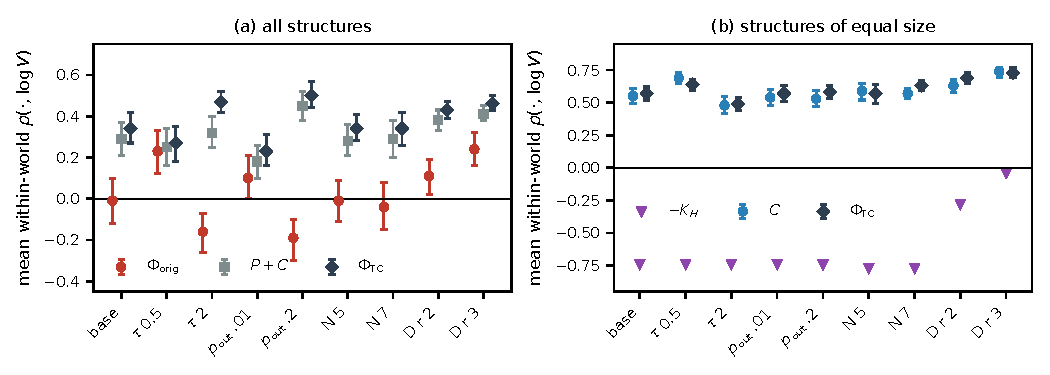
\includegraphics[width=\textwidth]{figures/fig_s1.pdf}
\caption{Robustness over nine settings (corrected code). (a) Over all structures, $\Phiorig$ (red) has an interval
above zero in 3 of 9 settings, while $P+C$ and the unit-free $\PhiTC$ are above zero in all 9. (b) Among structures of
equal size, memory $C$ and $\PhiTC$ predict $\log V$ in all settings. The entropy term $-K_H$ predicts life in the
wrong direction when $D=I$, and the effect disappears when the D-test unties variance from time scale.
Bars: 95\% cluster-bootstrap intervals over 90 worlds.}
\label{fig:s1}
\end{figure}

\subsection{A complexity term free of units}
$K_H = h(A_t)$ changes by $\log c_i$ when a variable $x_i$ is rescaled by $c_i$. Different structures hold different
variables, so the ranking by $\Phiorig$ depends on an arbitrary choice of units, while $P$, $C$ and $V$ do not. S1b
replaces $K_H$ by the total correlation $\TC$, which uses only correlations:
\begin{equation}
  \PhiTC = P + C - 0.25\,\TC ,
\end{equation}
with the weights of $\Phiorig$ and no tuning. A test confirms that the ranking by $\PhiTC$ does not change under random
rescaling, while the ranking by $\Phiorig$ does. $\PhiTC$ predicts viability in all 9 settings ($\rho$ from $+0.23$ to
$+0.50$, Fig.~\ref{fig:s1}a). It is above $P+C$ in 9 of 9 settings, and the coefficient of $\TC$ in the regression is
negative in all three families of all 9 settings. Internal integration is a cost for persistence here.

One
pre-registered rule failed: $\PhiTC$ is not stable under the D-test, because its $\rho$ moves by $+0.12$ between the
baseline and $r=3$ (limit 0.1). We had expected $\TC$ to fix the $\tau$ dependence only in part, and the $\tau$ settings
still disagree ($+0.27$ to $+0.47$).

\subsection{Merging}
\label{sec:merge}
For two disjoint structures, $h(A\cup B) = h(A) + h(B) - I(A;B)$, so
$\Delta\Phi = \Phi(A\cup B) - \Phi(A) - \Phi(B) = \Delta P + \beta\Delta C + \lambda I(A;B)$. H4 asked whether
$\Delta\Phi$ predicts the survival synergy $S = V_{A\cup B}(1/V_A + 1/V_B)$ better than the static dependence
$I(A;B)$. Over all 24\,300 pairs it does not: $\rho(\Delta\Phi, \log S) = -0.17$ [$-0.23$, $-0.11$], against $+0.36$
[$+0.32$, $+0.40$] for $I(A;B)$ alone. The $P$ term points the wrong way, because a merger shrinks the environment and
so lowers $P$. In 77\% of pairs the union lives longer than the two parts in parallel ($S>1$).

\subsection{Growth rate as viability}
S4 replaces the mean exit time by a population growth rate $r$. Every structure gives birth at rate $b=1$ from a
maturation age $a_m$ on, and $r$ solves the Euler--Lotka equation \cite{Lotka1907,Charlesworth94}
\begin{equation}
  1 = b\int_{a_m}^{\infty} e^{-ra}\,l(a)\,\mathrm{d}a ,
\end{equation}
with $l(a)$ the survival curve of the structure. One birth rule for all structures keeps the answer out of the rule:
$r$ differs from $V$ only through the shape of $l(a)$. Lives are close to exponential (median coefficient of variation
1.04), so $r$ ranks structures like $V$ ($\rho = 0.95$ at $a_m=0$, $0.99$ at $a_m$ equal to the median $V$). $V$ is the
slightly more stable ranking when $\pout$ changes from 0.05 to 0.2. $\PhiTC$ predicts $r$ ($+0.35$ [$+0.29$, $+0.41$]).
With an offspring map that swaps one variable at rate 0.1, the Price selection term on $\PhiTC$ is positive in 74\% of
worlds and the transmission term is small and negative in 98\%.

\section{What a functional must also capture}

\subsection{Drive-sustained versus passive persistence}
\label{sec:flux}
A bistable ``rock'' at equilibrium has a long memory of its well, but it does nothing to stay alive. S2 builds units with
state $z=(x,v)$:
\begin{equation}
  \mathrm{d}x = v\,\mathrm{d}t, \qquad \mathrm{d}v = \bigl(-U'(x) - \gamma(v)\,v\bigr)\mathrm{d}t + \sqrt{2\gamma_0 T}\,\mathrm{d}W ,
\end{equation}
with $\gamma_0=1$ and $T=0.1$. Rocks have $U = h(x^2-1)^2$ and constant friction. Oscillators have
$U = \omega_0^2 x^2/2$ and the active Rayleigh friction $\gamma(v) = \gamma_0 - \alpha + \beta v^2$ of the
energy-depot model \cite{SchweitzerEbelingTilch98,Romanczuk12}: at low speed the friction is negative and the drive
pumps energy in. With the drive off ($\gamma = \gamma_0$) every unit relaxes to the Boltzmann law \cite{Kramers40}.
A drive alone cannot create a cycle in an overdamped system with a convex potential (Bendixson criterion), which is why
we use inertial units. $V$ is the mean exit time from the 95\% highest-density region of the unit's own stationary law.
$C$ and $\TC = I(x;v)$ come from the Kraskov--St\"ogbauer--Grassberger estimator \cite{Kraskov04}. The flux ratio
$\Von/\Voff$ needs a second simulation with the drive off.

At $\tau=1$ (S2), the flux cut shortens every oscillator's life by a median factor of 5.5 and leaves passive units
unchanged, and $C$ rates every oscillator above every rock. A post-hoc check showed that this rock class is a weak test. Rocks mostly leave through the outer edge of the set, and $C$ at $\tau=1$ measures motion inside the well.

S2b therefore
redefines viability as memory. A rock is alive while it stays in its well. An oscillator is alive while its
energy stays above a quarter of its cycle energy. We measure $C$ at a common long lag $\tau^\ast$, the median rock life.
The flux cut then shortens oscillator life about 23 times. In the first draw of units, $C(\tau^\ast)$ rated rocks above
oscillators of equal life (stratified AUC 0.76 [0.60, 0.86]), which triggered the pre-registered gate ``add a
dissipation term''. A replicate with new units did not repeat this (0.46). Over 7 independent draws the pooled AUC is
0.57 [0.51, 0.65], and the gate triggers in 2 of 7 draws. So memory does rate passive rocks slightly above driven
oscillators at a long lag, but the effect is weak.

With each unit's own lag, $C$ favours oscillators (AUC 0.18). The finding that holds in every draw is that $C$ alone cannot tell drive-sustained persistence from passive memory, while the flux ratio
can. A check at half the time step gave the same verdicts.

\paragraph{A dissipation term (S2c).} The direct candidate is the dissipation of the structure. Among oscillators the
drive power tracks life ($\rho = +0.70$ [$+0.55$, $+0.80$]) and drive dependence ($+0.58$).

In linear worlds, adding
$\sigma_A\tau$ to $\PhiTC$ lowers its ranking quality ($\Delta\rho = -0.19$ [$-0.25$, $-0.13$] in the baseline, $-0.54$
in the D-test with $r=3$). The direct link between $\sigma_A$ and life is null in the baseline ($+0.09$ [$-0.01$,
$+0.19$]) and negative in the D-test ($-0.27$). So raw dissipation is not a good general term: it helps where the drive
builds the structure and hurts where the drive only stirs it.

\subsection{Information that is used}
\label{sec:agency}
In passive worlds nothing uses predictive information, which may explain the small effect of $P$. S3 builds a linear
homeostat: a hidden environmental state $h$ (time scale $T_h\in[2,20]$), a sensor $s$, a memory $m$, an actuator $u$
with loop gain $L$, and a viability variable $v$ that $h$ pushes and $u$ can push back. The organism $A=\{s,m,u,v\}$ is
alive while $|v|<c$, with $c$ fixed for each organism. All information terms stay exact. Each of 400 organisms runs in
three versions: intact, \emph{scrambled} and without feedback. In the scrambled version the actuator reads a copy of the
memory that an independent copy of the environment drives. This input has the same statistics but no information about
$h$ \cite{KolchinskyWolpert18}. This is the full scrambling intervention of semantic information
\cite{KolchinskyWolpert18,Sowinski23}. So the VoI below is the viability value of all the information about $h$, and we
do not search for the smallest amount that keeps the viability.

The value of information $\mathrm{VoI} = \log V_{\mathrm{intact}} - \log V_{\mathrm{scrambled}}$ is $+1.27$ [$+1.14$,
$+1.40$] on average and positive in 99\% of organisms, so breaking the sensor--actuator link shortens life about
3.5 times (Fig.~\ref{fig:s3}). The effect of $P$ on $\log V$ depends on the loop: the standardised coefficient is
$+0.76$ with a working loop and $+0.37$ with a scrambled one (difference $+0.38$ [$+0.25$, $+0.52$]). Organisms with more
predictive information lose more when the loop is cut ($\rho(P,\mathrm{VoI}) = +0.41$).

The expected good-regulator
pattern \cite{ConantAshby70,TouchetteLloyd00}, a negative link between $I(v_t;h_t)$ and life, does not appear
($+0.30$), and a lagged version does not show it either. $\PhiTC$ ranks intact organisms ($+0.21$) but less well than
scrambled ones ($+0.39$): with a working loop, the quality of the loop matters, and $\PhiTC$ does not measure it.
The result is the same at half the time step.

\begin{figure}[t]
\centering
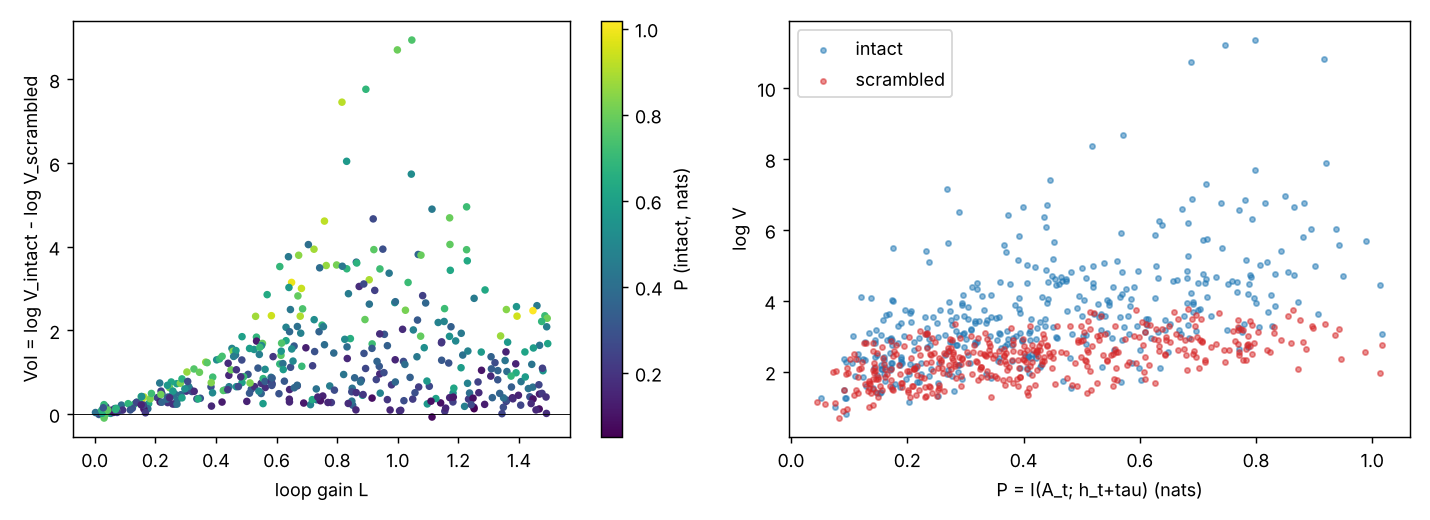
\includegraphics[width=0.95\textwidth]{figures/fig_s3.png}
\caption{Information that is used (S3, 400 homeostats, corrected code). Left: value of information against the loop
gain $L$, coloured by the predictive information $P$. Right: $\log V$ against $P$ for intact (blue) and scrambled (red)
organisms. The same predictive information buys a longer life only when the loop uses it.}
\label{fig:s3}
\end{figure}

\subsection{Boundaries by conditional independence}
\label{sec:blankets}
A functional of a structure needs the structure. S5 plants two structures in worlds of 24 variables. Each has an
interior of 3 variables and a blanket of 3 variables that couple the interior to a random background. No variable has
a special drive or noise. A \emph{static} detector uses zeros of the precision matrix \cite{Pearl88,Friston13}. A
\emph{dynamic} detector uses zeros of the drift matrix, estimated with the matrix logarithm $\hat B = -\log\bigl(\hat C(\Delta)\hat S^{-1}\bigr)/\Delta$,
which is exact for exact covariances. In equilibrium worlds both detectors recover all 80 planted blankets. In driven
worlds the stationary precision matrix is dense, as Aguilera et al.\ predict \cite{AguileraMillidgeTschantzBuckley22}.
With exact covariances the static detector recovers none. With a calibrated threshold on finite data it recovers 99\%,
because the extra terms are small. When we double and quadruple the drive, static recovery falls to 0.84 and 0.46,
while the dynamic blanket stays exact.

Total correlation and closure rank the planted interiors in the top 2\% of all
candidate structures, while $\PhiTC$ ranks them near the bottom (percentile 0.02 to 0.04). The score that predicts
persistence in passive worlds is the wrong score to find structures.

\section{Replication, heredity and selection}
\label{sec:spots}
T3 needs a transmission term, which needs division. S6 uses Gray--Scott self-replicating spots \cite{Pearson93},
\begin{equation}
  u_t = D_u\nabla^2 u - uv^2 + F(1-u), \qquad v_t = D_v\nabla^2 v + uv^2 - (F + k - \varepsilon a)v ,
\end{equation}
with $D_u = 0.16$, $D_v = 0.08$, $F = 0.0367$, $k = 0.0649$, explicit Euler steps on a periodic grid and small noise on
$v$. Two dyes $a$ and $b$ compete inside spots, $a_t = D_c\nabla^2 a + \gamma s\,a(1-a-2b) - \delta(1-s)a$ (and the
same with $a$ and $b$ swapped), so each spot settles on one heritable type. Type A lowers the local kill rate by
$\varepsilon a$. A tracker links spots across frames by overlap and records each division. We compute the Price terms
\cite{Price70,Frank95}
\begin{equation}
  \bar w\,\Delta\bar z = \mathrm{Cov}(w, z) + \mathrm{E}[w\,\Delta z]
\end{equation}
per generation, with $z = 1$ for type A and $w$ the number of daughters that divide again.

\paragraph{First test bed.} With a neutral dye, spots replicate from 4 to about 230 and the pipeline measures
heredity (parent--daughter $\rho = 0.975$). But the pooled selection term on the neutral trait is $+4.72$ instead of 0,
mostly because pooling mixes generations. So Price terms need per-generation bookkeeping and a neutral control.

\paragraph{Selection (S6b).} With $\varepsilon = 0.001$ type A divides 24\% faster. In 32 colonies on a $300\times300$
grid the per-generation selection term is $+0.041$ [$+0.038$, $+0.044$], and type A rises to 72\%. The neutral control
($\varepsilon=0$, 32 colonies) gives a selection term consistent with 0 and a final fraction of 0.50. Fidelity is 1.000,
so the transmission term is 0. Colony growth is polynomial (power-law exponent 1.92), as expected when only part of
a colony has free space.

\paragraph{Mutation and the error threshold (S6c--S6f).} At each division a type-A daughter becomes type B with
probability $\mu$. The measured mutation rate equals the set rate at all 9 values of $\mu$. The transmission term,
counted over all daughters, matches $-\mu\,\mathrm{E}[wz]/\bar w$ within about 3\%. (The pre-registered version counted
only daughters that divide again and gave 50--60\% of the prediction. Mutant daughters divide less often before the run
ends, so this rule failed for a bookkeeping reason.) From the cycle times in S6b, a mean-field single-peak model predicts
an error threshold at $\mu_c = 1 - 2^{T_A/T_B-1} = 0.114$ \cite{Eigen71}.

The colonies show no sharp threshold
(Fig.~\ref{fig:s6}): the final fraction of type A falls smoothly and crosses 0.1 only at $\mu\approx0.32$, about 3 times
$\mu_c$. A finite-time mean field keeps much less type A (0.27 against 0.58 at $\mu_c$), so the spatial colony protects
the faster type. On a $600\times600$ grid with about twice the generations (S6d), the fraction falls further above
$\mu_c$ (0.16 at $2\mu_c$) and holds below it, but the change stays gradual. We expected the protection to come from
the colony edge.

A direct test (S6e) did not support this: divisions lean only a little toward the edge (AUC 0.57), and
type A sits \emph{inside} the colony (AUC 0.32 for being nearer the edge than type B). A rerun with a corrected GPU
noise generator (S6f) gave the same verdicts.

\begin{figure}[t]
\centering
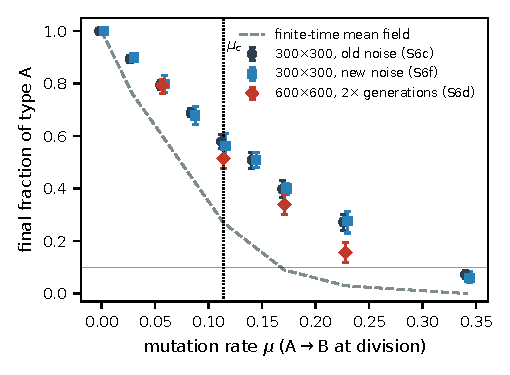
\includegraphics[width=0.6\textwidth]{figures/fig_s6.pdf}
\caption{Final fraction of the faster type against the mutation rate. Circles and squares: $300\times300$ colonies with
the old and the corrected GPU noise (20 and 10 colonies per $\mu$). Diamonds: $600\times600$ colonies with about twice
the generations (8 per $\mu$). Dashed: finite-time mean field with the same run length. The dotted line marks the
mean-field threshold $\mu_c = 0.114$. Bars: 95\% bootstrap intervals over colonies.}
\label{fig:s6}
\end{figure}

\section{Numerical audit and reruns}
\label{sec:audit}
After S6 we reviewed the numerical code against the documentation and found 13 problems. Table~\ref{tab:audit} lists
the ones that could change a result. Two were serious. First, the exit check on the time grid made $\log V$ too high by $+0.2$ to $+1.2$, and more for fast structures. So it changed the ranking of structures (Spearman 0.85 to 0.98 between
$\mathrm{d}t=0.05$ and $\mathrm{d}t=0.005$). The original documentation said that the bias was the same for every
structure, which was wrong. Second, a filter in the merge analysis dropped 54\% of the eligible pairs, and the dropped
pairs depended on the variable index.

We fixed every problem, reran every affected step on the same seeds, and wrote
the rerun rules before the reruns. No main conclusion changed. Effect sizes moved: the regression coefficients of
H2 grew by 20--100\% because the old check compressed the differences between fast and slow structures. Three verdicts changed. H1 became supported in the D-test with $r=2$, H2 at $\tau=2$ became ``partial'' (it was ``not supported''),
and the S2c link between dissipation and life in the baseline became null (it was weakly positive). A rerun of the
corrected baseline on a second machine gave the same point estimates, with differences below $10^{-15}$.

\begin{table}[t]
\centering
\small
\caption{Problems found by the numerical audit that could change a result, and their effect after the rerun.}
\label{tab:audit}
\begin{tabular}{@{}p{5.6cm} p{3.4cm} p{4.4cm}@{}}
\toprule
Problem & Fix & Effect on conclusions \\
\midrule
Exit check misses excursions; bias grows with the relaxation rate & Brownian-bridge correction & None changed; effect sizes 20--100\% larger; 3 verdicts changed (see text) \\
Merge analysis dropped 54\% of pairs & All 24\,300 pairs & H4 still fails in all 9 settings \\
Equilibrium control without common random numbers & Common random numbers & Control exact ($\log R = 0$) \\
KSG used above its validated range & Validation at 2--3 nats in 4 dimensions & Error at most 6.7\%; no rerun needed \cite{Gao15} \\
Price-identity check true by construction & Restated as an arithmetic check & None \\
GPU noise repeats at some time lags & 64-bit counter-based hash & S6b and S6c verdicts unchanged \\
\bottomrule
\end{tabular}
\end{table}

\section{Discussion}

\subsection{What supports an arrow of organisation}
We fixed four conditions for support of T3 before the experiments. Table~\ref{tab:t3} gives the result.

\begin{table}[t]
\centering
\small
\caption{The four pre-registered conditions for support of T3.}
\label{tab:t3}
\begin{tabular}{@{}p{5.2cm} p{1.6cm} p{6.6cm}@{}}
\toprule
Condition & Verdict & Evidence \\
\midrule
1. $\Phi$-like scores predict viability, also after a flux cut & in part & $C$ and $\PhiTC$ in 9 of 9 linear settings; $\Phiorig$ in 3 of 9; $C$ alone does not separate driven from passive persistence \\
2. Information that is used pays & yes & VoI $+1.27$; the effect of $P$ depends on the loop \\
3. A positive Price selection term & yes & Spot colonies with a heritable type; $\PhiTC$ in linear worlds (74\% of worlds) \\
4. A measured, nonzero transmission term & yes & One-way mutation at division; the term matches the mutation rate \\
\bottomrule
\end{tabular}
\end{table}

The pattern is consistent. Persistence in these systems rewards memory and penalises internal integration, and
predictive information pays only through action. The original functional mixes these with a complexity term that has
no physical meaning across structures, and it fails. A unit-free variant succeeds in passive linear worlds, but the same
variant is the wrong score to find structures and cannot tell a dissipative structure from a passive memory. So T2, in
the form of one functional that organisations extremise, has no support here. T3 has partial support. Selection on a heritable organisational trait and transmission with copying errors are
both measurable, and they behave as the Price equation says. But the trait in the spot colonies is a designed type, not an information score.

\subsection{Limitations}
The linear worlds are small ($N\le 7$) and Gaussian, so every information term is exact, but none of them has an action
loop or real division. The homeostat is linear, with a Gaussian hidden state. The nonlinear units are one-dimensional
oscillators, and their information terms come from an estimator. The spot colonies divide only where there is free
space, and runs end when the grid is full, after at most about 30 generations. Pre-registration was self-administered.
Several design choices (the families, the viability set, the offspring map of S4, the birth rule, the mutation scheme)
are ours, and other choices can give other answers. Growing and dividing active droplets \cite{Zwicker17} are a
natural next test bed, because their division comes from a physical growth mechanism.

\subsection{Open questions}
\begin{enumerate}
  \item Is there one score that predicts persistence in passive, driven and agentic systems, and that also finds
  structures? The best candidate here, $\PhiTC$, is tested only in linear worlds.
  \item Can a closed-form term capture ``dissipation that builds the structure'' without a drive-off simulation?
  \item Why does the faster type survive better in spatial colonies than in mean field, if it does not stay at the edge?
  A post-hoc reading is that divisions, and therefore new mutants, lean toward the front, while old type-A spots remain
  in the interior. We did not test this.
  \item Does a sharp error threshold appear with many more generations, for example on larger grids or in colonies
  that remove spots?
  \item Does the dynamic Markov blanket, which stays exact under drive, give better candidate structures for a
  functional than conditional independence in the stationary law?
  \item How does $\PhiTC$ compare with semantic information \cite{KolchinskyWolpert18,Bartlett25} on the same
  structures? A fixed score is cheap to compute. Semantic information needs interventions, but it measures use directly.
\end{enumerate}

\section{Conclusions}
The original information functional of the variational proposal does not predict the persistence of structures in
random linear worlds. Its verdict depends on the lag and on the noise structure, and its complexity term depends on the
units. Memory and a unit-free variant with a total-correlation penalty predict persistence in all nine settings we
tested. Memory alone cannot tell a drive-sustained structure from a passive one, while a flux cut can. Predictive
information extends life only when an action loop uses it. In self-replicating spot colonies, per-generation Price
terms with a neutral control measure both selection and a transmission term from copying errors, but space blurs the
mean-field error threshold. An arrow of organisation therefore has partial support in these model systems, and a single
variational functional of life has none so far.

\section*{Data and code availability}
All code, the pre-registered rules, the step documents, the reports, the logs and the numerical audit are public at
\url{https://github.com/PepeDest/Beiro-Feat-Flutter-Big-ass-project}. The simulation data (about 250\,MB) are not in the
repository. The README gives the commands to regenerate them with fixed seeds. The test suite has 75 tests. The GPU code
needs OpenCL with double precision.

\section*{Use of generative AI}
The code, the simulations, the analyses and a first draft of this text were produced with substantial help from Claude
(Anthropic), a generative AI model, under the direction of the author. The author takes full responsibility for all contents of this paper.

\bibliographystyle{unsrtnat}
\bibliography{refs}

\end{document}
